%!TEX encoding = UTF-8 Unicode
\documentclass[french]{article}



%% Langue et compilation

\usepackage[utf8]{inputenc}
\usepackage[T1]{fontenc}
\usepackage[french]{babel}

%% LISTE DES PACKAGES

\usepackage{mathtools}     % package de base pour les maths
\usepackage{amsmath}       % mathematical type-setting
\usepackage{amssymb}       % symbols speciaux pour les maths
\usepackage{textcomp}      % symboles speciaux pour el text
\usepackage{gensymb}       % commandes generiques \degree etc...
\usepackage{tikz}          % package graphique
\usepackage{wrapfig}       % pour entourer a cote d'une figure
\usepackage{color}         % package des couleurs
\usepackage{xcolor}        % autre package pour les couleurs
\usepackage{pgfplots}      % pacakge pour creer des graph
\usepackage{epsfig}        % permet d'inclure des graph en .eps
\usepackage{graphicx}      % arguments dans includegraphics
\usepackage{pdfpages}      % permet d'insérer des pages pdf dans le document
\usepackage{subfig}        % permet de creer des sous-figure
\usepackage{pst-all}       % utile pour certaines figures en pstricks
\usepackage{lipsum}        % package qui permet de faire des essais
\usepackage{array}         % permet de faire des tableaux
\usepackage{multicol}      % plusieurs colonnes sur une page
\usepackage{enumitem}      % pro­vides user con­trol: enumerate, itemize and description
\usepackage{hyperref}      % permet de creer des hyperliens dans le document
\usepackage{lscape}        % permet de mettre une page en mode paysage
\usepackage{lmodern}       % permet d'avoir certains "fonts" de bonen qualite
\usepackage{fancyhdr}      % Permet de mettre des informations en hau et en bas de page      
\usepackage[framemethod=tikz]{mdframed} % breakable frames and coloured boxes
\usepackage[top=1.5cm, bottom=1.5cm, left=2.5cm, right=2.5cm]{geometry} % donne les marges
\usepackage[font=normalsize, labelfont=bf,labelsep=endash, figurename=Fig.]{caption} % permet de changer les legendes des figures
\usepackage{lewis}
\usepackage{bohr}
\usepackage{chemfig}
\usepackage{chemist}

%% LIBRAIRIES

\usetikzlibrary{plotmarks} % librairie pour les graphes
\usetikzlibrary{patterns}  % necessaire pour certaines choses predefinies sur tikz
\usetikzlibrary{shadows}   % ombres des encadres
\usetikzlibrary{backgrounds} % arriere plan des encadres


%% MISE EN PAGE

\pagestyle{fancy}     % Défini le style de la page

\renewcommand{\headrulewidth}{1pt}      % largeur du trait en haut de la page
\fancyhead[L]{Seconde générale}         % info coin haut gauche
\fancyhead[R]{Lycée Jean Guéhenno}  % info coin haut droit

% bas de la page
\renewcommand{\footrulewidth}{1pt}      % largeur du trait en bas de la page
\fancyfoot[L]{G. \bsc{LE DOUDIC}}  % info coin bas gauche
\fancyfoot[R]{TP 4 : Famille chimique}                         % info coin bas droit


\setlength{\columnseprule}{1pt} 
\setlength{\columnsep}{30pt}



%% NOUVELLES COMMANDES 

\DeclareMathOperator{\e}{e} % permet d'ecrire l'exponentielle usuellement


\newcommand{\gap}{\vspace{0.15cm}}   % defini une commande pour sauter des lignes
\renewcommand{\vec}{\overrightarrow} % permet d'avoir une fleche qui recouvre tout le vecteur
\newcommand{\bi}{\begin{itemize}}    % begin itemize
\newcommand{\ei}{\end{itemize}}      % end itemize
\newcommand{\bc}{\begin{center}}     % begin center
\newcommand{\ec}{\end{center}}       % end center
\newcommand\opacity{1}               % opacity 
\pgfsetfillopacity{\opacity}

\newcommand*\Laplace{\mathop{}\!\mathbin\bigtriangleup} % symbole de Laplace

\frenchbsetup{StandardItemLabels=true} % je ne sais plus

\newcommand{\smallO}[1]{\ensuremath{\mathop{}\mathopen{}o\mathopen{}\left(#1\right)}} % petit o

\newcommand{\cit}{\color{blue}\cite} % permet d'avoir les citations de couleur bleues
\newcommand{\bib}{\color{black}\bibitem} % paragraphe biblio en noir et blanc
\newcommand{\bthebiblio}{\color{black} \begin{thebibliography}} % idem necessaire sinon bug a cause de la couleur
\newcommand{\ethebiblio}{\color{black} \end{thebibliography}}   % idem
%%% TIKZ


%% COULEURS 


\definecolor{definitionf}{RGB}{220,252,220}
\definecolor{definitionl}{RGB}{39,123,69}
\definecolor{definitiono}{RGB}{72,148,101}

\definecolor{propositionf}{RGB}{255,216,218}
\definecolor{propositionl}{RGB}{38,38,38}
\definecolor{propositiono}{RGB}{109,109,109}

\definecolor{theof}{RGB}{255,216,218}
\definecolor{theol}{RGB}{160,0,4}
\definecolor{theoo}{RGB}{221,65,100}

\definecolor{avertl}{RGB}{163,92,0}
\definecolor{averto}{RGB}{255,144,0}

\definecolor{histf}{RGB}{241,238,193}

\definecolor{metf}{RGB}{220,230,240}
\definecolor{metl}{RGB}{56,110,165}
\definecolor{meto}{RGB}{109,109,109}


\definecolor{remf}{RGB}{230,240,250}
\definecolor{remo}{RGB}{150,150,150}

\definecolor{exef}{RGB}{240,240,240}

\definecolor{protf}{RGB}{247,228,255}
\definecolor{protl}{RGB}{105,0,203}
\definecolor{proto}{RGB}{174,88,255}

\definecolor{grid}{RGB}{180,180,180}

\definecolor{titref}{RGB}{230,230,230}

\definecolor{vert}{RGB}{23,200,23}

\definecolor{violet}{RGB}{180,0,200}

\definecolor{copper}{RGB}{217, 144, 88}

%% Couleur des ref

\hypersetup{
	colorlinks=true,
	linkcolor=black,
	citecolor=blue,
	urlcolor=black
		   }

%% CADRES


% %%%%%%%%%% DEFINITION
% \newmdenv[tikzsetting={fill=definitionf}, linewidth=2pt, linecolor=definitionl, outerlinewidth=0pt, innertopmargin=5pt, innerbottommargin=5pt, innerleftmargin=5pt, innerrightmargin=5pt, leftmargin=0pt]{definition}

% \newmdenv[ tikzsetting={drop shadow={ shadow xshift=1ex, shadow yshift=-0.5em, fill=definitiono, opacity=1, every shadow } }, outerlinewidth=2pt, outerlinecolor=white, linecolor=white, innertopmargin=0pt, innerbottommargin=0pt, innerleftmargin=0pt, innerrightmargin=0pt]{ombredef}


% %%%%%%%%%% THEOREME

% \newmdenv[tikzsetting={fill=theof}, linewidth=2pt, linecolor=theol, outerlinewidth=0pt, innertopmargin=5pt, innerbottommargin=5pt, innerleftmargin=5pt, innerrightmargin=5pt, leftmargin=0pt]{theo}

% \newmdenv[ tikzsetting={drop shadow={ shadow xshift=1ex, shadow yshift=-0.5em, fill=theoo, opacity=1, every shadow } }, outerlinewidth=2pt, outerlinecolor=white, linecolor=white, innertopmargin=0pt, innerbottommargin=0pt, innerleftmargin=0pt, innerrightmargin=0pt]{ombretheo}


% %%%%%%%%%% METHODE

% \newmdenv[tikzsetting={fill=metf}, linewidth=2pt, linecolor=metl, outerlinewidth=0pt, innertopmargin=5pt, innerbottommargin=5pt, innerleftmargin=5pt, innerrightmargin=5pt, leftmargin=0pt]{met}

% \newmdenv[ tikzsetting={drop shadow={ shadow xshift=1ex, shadow yshift=-0.5em, fill=meto, opacity=1, every shadow } }, outerlinewidth=2pt, outerlinecolor=white, linecolor=white, innertopmargin=0pt, innerbottommargin=0pt, innerleftmargin=0pt, innerrightmargin=0pt]{ombremet}



%%%%%%%%%%% RQ

\newmdenv[tikzsetting={fill=remf}, linewidth=2pt, linecolor=remf, outerlinewidth=0pt, innertopmargin=5pt, innerbottommargin=5pt, innerleftmargin=5pt, innerrightmargin=5pt, leftmargin=0pt]{remarque}

\newmdenv[ tikzsetting={drop shadow={ shadow xshift=1ex, shadow yshift=-0.5em, fill=remo, opacity=1, every shadow } }, outerlinewidth=2pt, outerlinecolor=white, linecolor=white, innertopmargin=0pt, innerbottommargin=0pt, innerleftmargin=0pt, innerrightmargin=0pt]{ombreremarque}

%%%%%%%%%%% Cadre pour le titre

\tikzset{every shadow/.style={opacity=1}}

\global\mdfdefinestyle{doc}{backgroundcolor=white, shadow=true, shadowcolor=propositiono, linewidth=1pt, linecolor=black, shadowsize=5pt}
\global\mdfdefinestyle{titr}{backgroundcolor=metf, shadow=true, shadowcolor=propositiono, linewidth=1pt, linecolor=black, shadowsize=5pt}
\global\mdfdefinestyle{theo}{backgroundcolor=theof, shadow=true, shadowcolor=theoo, linewidth=1pt, linecolor=theol, shadowsize=5pt}
\global\mdfdefinestyle{prop}{backgroundcolor=theof, shadow=true, shadowcolor=propositiono, linewidth=1pt, linecolor=theol, shadowsize=5pt}
\global\mdfdefinestyle{def}{backgroundcolor=definitionf, shadow=true, shadowcolor=definitiono, linewidth=1pt, linecolor=definitionl, shadowsize=5pt}
\global\mdfdefinestyle{histo}{backgroundcolor=histf, shadow=true, shadowcolor=propositiono, linewidth=1pt, linecolor=black, shadowsize=5pt}
\global\mdfdefinestyle{avert}{backgroundcolor=white, shadow=true, shadowcolor=averto, linewidth=1pt, linecolor=avertl, shadowsize=5pt}
\global\mdfdefinestyle{met}{backgroundcolor=metf, shadow=true, shadowcolor=meto, linewidth=1pt, linecolor=metl, shadowsize=5pt}
\global\mdfdefinestyle{rem}{backgroundcolor=metf, shadow=true, shadowcolor=meto, linewidth=1pt, linecolor=metf, shadowsize=5pt}
\global\mdfdefinestyle{exo}{backgroundcolor=exef, shadow=true, shadowcolor=propositiono, linewidth=1pt, linecolor=exef, shadowsize=5pt}
\global\mdfdefinestyle{not}{backgroundcolor=definitionf, shadow=true, shadowcolor=propositiono, linewidth=1pt, linecolor=black, shadowsize=5pt}
\global\mdfdefinestyle{proto}{backgroundcolor=protf, shadow=true, shadowcolor=proto, linewidth=1pt, linecolor=protl, shadowsize=5pt}

%%%%%%
\definecolor{cobalt}{rgb}{0.0, 0.28, 0.67}
\definecolor{applegreen}{rgb}{0.55, 0.71, 0.0}

\usepackage{tcolorbox}
  \tcbuselibrary{most}
  \tcbset{colback=cobalt!5!white,colframe=cobalt!75!black}



\newtcolorbox{definition}[1]{
	colback=applegreen!5!white,
  	colframe=applegreen!65!black,
	fonttitle=\bfseries,
  	title={#1}}
\newtcolorbox{Programme}[1]{
	colback=cobalt!5!white,
  	colframe=cobalt!65!black,
	fonttitle=\bfseries,
  	title={#1}}  

\newtcolorbox{Exercice}[1]{
  colback=cobalt!5!white,
  colframe=cobalt!65!black,
  fonttitle=\bfseries,
  title={#1}}  

  \newtcolorbox{Protocol}[1]{
  colback=cyan!5!white,
  colframe=cyan!65!black,
  fonttitle=\bfseries,
  title={#1}}  

\newtcolorbox{Resultat}[1]{
	colback=theof,%!5!white,
	colframe=theoo!85!black,
  fonttitle=\bfseries,
	title={#1}} 	


\def\width{12}
\def\hauteur{5}

\setlength{\parskip}{0pt}%
\setlength{\parindent}{18pt}


%% MODIFICATION DE CHAPTER  
\makeatletter
\def\@makechapterhead#1{%
  %%%%\vspace*{50\p@}% %%% removed!
  {\parindent \z@ \raggedright \normalfont
    \ifnum \c@secnumdepth >\m@ne
        \huge\bfseries \@chapapp\space \thechapter
        \par\nobreak
        \vskip 20\p@
    \fi
    \interlinepenalty\@M
    \Huge \bfseries #1\par\nobreak
    \vskip 40\p@
  }}
\def\@makeschapterhead#1{%
  %%%%%\vspace*{50\p@}% %%% removed!
  {\parindent \z@ \raggedright
    \normalfont
    \interlinepenalty\@M
    \Huge \bfseries  #1\par\nobreak
    \vskip 40\p@
  }}
  
  \newcommand{\isotope}[3]{%
     \settowidth\@tempdimb{\ensuremath{\scriptstyle#1}}%
     \settowidth\@tempdimc{\ensuremath{\scriptstyle#2}}%
     \ifnum\@tempdimb>\@tempdimc%
         \setlength{\@tempdima}{\@tempdimb}%
     \else%
         \setlength{\@tempdima}{\@tempdimc}%
     \fi%
    \begingroup%
    \ensuremath{^{\makebox[\@tempdima][r]{\ensuremath{\scriptstyle#1}}}_{\makebox[\@tempdima][r]{\ensuremath{\scriptstyle#2}}}\text{#3}}%
    \endgroup%
  }%

\makeatother

\usepackage{lewis}
\usepackage{bohr}
\usepackage{chemfig}
\usepackage{chemist}
\usepackage{tabularx}

% %%% TEST EXERCIES SOLUTIONS
% \usepackage{answers}
% %\usepackage[nosolutionfiles]{answers}
% % def d'un environnement Exercise numerote
% \newtheorem{Exc}{Exercise}
% \newenvironment{Ex}{\begin{Exc}\normalfont}%
%                    {\end{Exc}}
% % Trois types de solutions sont proposes
% \Newassociation{solution}{Soln}{test}
% \Newassociation{hint}{Hint}{test}
% \Newassociation{Solution}{sSol}{testtwo}
% \newcommand{\prehint}{~[Hint]}
% \newcommand{\presolution}{~[Solution]}
% \newcommand{\preSolution}{~[Homework]}
% % test
% \newcommand{\Opentesthook}[2]%
%    {\Writetofile{#1}%
%     {\protect\section{#1: #2}}}
% % introduction de la solution
% \renewcommand{\Solnlabel}[1]{\emph{Solution #1}}
% \renewcommand{\Hintlabel}[1]{\emph{Hint #1}}
% \renewcommand{\sSollabel}[1]{\emph{Solution to #1}}


%%
%%
%% DEBUT DU DOCUMENT
%%
\setlength{\tabcolsep}{20pt}

\renewcommand{\arraystretch}{2}
\begin{document}

\tikzset{every shadow/.style={opacity=1}}

\global\mdfdefinestyle{doc}{backgroundcolor=white, shadow=true, shadowcolor=propositiono, linewidth=1pt, linecolor=black, shadowsize=5pt}
\global\mdfdefinestyle{titr}{backgroundcolor=titref, shadow=true, shadowcolor=propositiono, linewidth=1pt, linecolor=black, shadowsize=5pt}
\global\mdfdefinestyle{theo}{backgroundcolor=theof, shadow=true, shadowcolor=theoo, linewidth=1pt, linecolor=theol, shadowsize=5pt}
\global\mdfdefinestyle{prop}{backgroundcolor=theof, shadow=true, shadowcolor=propositiono, linewidth=1pt, linecolor=theol, shadowsize=5pt}
\global\mdfdefinestyle{def}{backgroundcolor=definitionf, shadow=true, shadowcolor=definitiono, linewidth=1pt, linecolor=definitionl, shadowsize=5pt}
\global\mdfdefinestyle{histo}{backgroundcolor=histf, shadow=true, shadowcolor=propositiono, linewidth=1pt, linecolor=black, shadowsize=5pt}
\global\mdfdefinestyle{avert}{backgroundcolor=white, shadow=true, shadowcolor=averto, linewidth=1pt, linecolor=avertl, shadowsize=5pt}
\global\mdfdefinestyle{met}{backgroundcolor=metf, shadow=true, shadowcolor=meto, linewidth=1pt, linecolor=metl, shadowsize=5pt}
\global\mdfdefinestyle{rem}{backgroundcolor=metf, shadow=true, shadowcolor=meto, linewidth=1pt, linecolor=metf, shadowsize=5pt}
\global\mdfdefinestyle{exo}{backgroundcolor=exef, shadow=true, shadowcolor=propositiono, linewidth=1pt, linecolor=exef, shadowsize=5pt}
\global\mdfdefinestyle{not}{backgroundcolor=definitionf, shadow=true, shadowcolor=propositiono, linewidth=1pt, linecolor=black, shadowsize=5pt}
\global\mdfdefinestyle{proto}{backgroundcolor=protf, shadow=true, shadowcolor=proto, linewidth=1pt, linecolor=protl, shadowsize=5pt}

%%%%%%

\begin{center}
	\begin{mdframed}[style=titr, leftmargin=55pt, rightmargin=55pt, innertopmargin=8pt, innerbottommargin=8pt, innerrightmargin=10pt, innerleftmargin=10pt]
		
		
		\begin{center}
			\Large{\textbf{Chapitre 2: Atome, noyau et cortège}} \\
			\large{\textbf{TP3: \og{} La configuration électronique\fg{}  et TP4: \og{}Familles chimiques\fg{}}}
		\end{center}
	\end{mdframed}
\end{center}

\begin{figure}[ht]
	\centering
	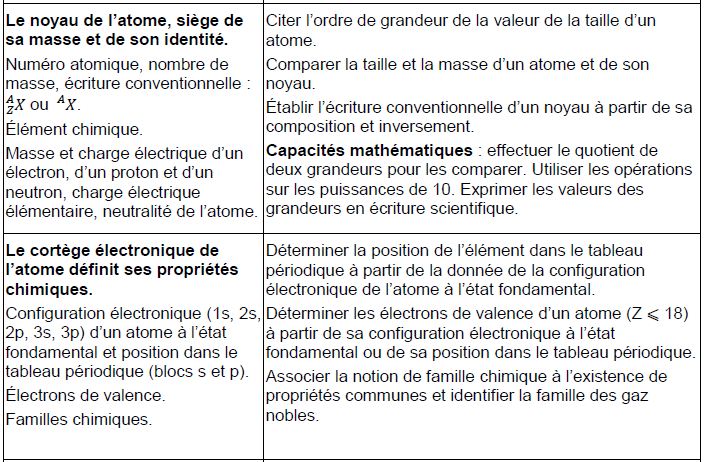
\includegraphics[width=1\textwidth]{BO.png}
	% \caption{Programme du chapitre}
\end{figure}
\begin{mdframed}[style=doc, leftmargin=0pt, rightmargin=0pt, innertopmargin=8pt, innerbottommargin=8pt, innerrightmargin=10pt, innerleftmargin=10pt]
		\noindent \textbf{Exercices}
\noindent \textbf{1. La description de l'atome}
		\begin{itemize}
			\item Composition d'un atome : 10, 12p80 
			\item Isotopes : 11p80 
			\item Calculer la masse d'un atome : 13p81
			\item Activité sur le modèle de l'atome : Histoire d'un modèle modèle de l'atome
		
		\end{itemize}
\noindent\textbf{2. Le cortège électronique}
\begin{itemize}
	\item Configurations électroniques : 12,13,14p98 et 15,17 p99
	\item Règle de l'octet : 5,7,8 p115
	\item Stabilité 10p115
	\item Représentation de Lewis 15p116
	\item Liaisons covalentes 21 p118
\end{itemize}
\end{mdframed}

% \begin{mdframed}[style=doc, leftmargin=0pt, rightmargin=0pt, innertopmargin=8pt, innerbottommargin=8pt, innerrightmargin=10pt, innerleftmargin=10pt]
% \noindent \textbf{Documents vidéos}

% \begin{figure}[ht]
	
% \end{figure}
% \subfloat[listentry][subcaption]{\includegraphics[options]{AgeDeLUniversCEADouVientLaMatiere.htm}}

% \end{mdframed}
\clearpage
\section*{Introduction}

D'où provient la matière qui nous entoure ? De quoi est-elle constituée ? Quel est le plus petit élément constitutif de la matière ? \medskip

Dès le cinquième siècle avant Jesus-Christ, Démocrite un philosphe grec s'interesse à la matière. D'après lui, la matière est faite de briques élémentaires incassables. Ce qu'il appelle des atomes (atomos en grec = insécable, qui ne peut pas être divisé). Les recherches sur ces briques élémentaires se poursuivent encore aujourd'hui avec de nombreux défis en particulier autour de l'énergie contenue dans la matière.\medskip

\begin{mdframed}[style=doc, leftmargin=0pt, rightmargin=0pt, innertopmargin=8pt, innerbottommargin=8pt, innerrightmargin=10pt, innerleftmargin=10pt]
\textbf{Document introductif : L'apparition de la matière}

Vidéo du Commissariat à l'Énergie Atomique (CEA). Il s'agit d'un organisme de recherche scientifique français dans les domaines de l'énergie, des sciences de la matière et de la santé. Un des principaux sites de recherche se trouve à l'Université Paris Saclay. \medskip

\url{https://www.youtube.com/watch?v=I-fWI6dKEys}


% \url{https://www.youtube.com/watch?v=fhaZeqzTVjo&ab_channel=CEA}

\end{mdframed}

\noindent\textbf{Questions en rapport avec la vidéo du CEA: }

\begin{enumerate}
	\item Quand apparaît la matière dans l'Univers ? 
	
	\textbf{Il y a $13,7$ Milliards d'années}%\dotfill

	\item Quel phénomène rend possible la fusion des particules ?
	
	\textbf{L'expansion de l'Univers entraîne son refroidissement. En refroidissant, les particules s'agitent moins et cela permet leur rencontre et leur fusion.}\bigskip

	\item De quoi sont formés les protons et les neutrons ?
	
	
	\textbf{Ils sont formés de Quarks}

	\item Comment nomme-t-on le phénomène qui donne naissance aux premiers atomes ?
	
	\textbf{Le phénomène qui donne lieu à la naissance des premiers atomes est la nucléosynthèse.}

\end{enumerate}



\section{La description de l'atome, un modèle}
\subsection{Qu'est-ce qu'un atome ? }

Les atomes peuvent être assimilés à des \textbf{sphères} avec un rayon de l'ordre de \textbf{$r_{\rm atome} = 0,1~\rm nm \text{ (nanomètres) }= 0,1\times 10^{-9}~\rm m$ } soit $10^{-10}$ mètres ($1\rm ~nm = 10^{-9} m$). Le rayon de l'atome est appelé \textbf{rayon atomique}.\medskip

Les atomes ne peuvent pas être vus à l'oeil nu ni au microscope optique. Les chercheurs sont aujourd'hui capables de détecter leur présence grâce aux microscopes à effet tunnel ou aux microscopes à force atomique.\medskip

\begin{definition}{Composition d'un atome}
	Un atome est constitué : 
	\begin{itemize}
		% \item \dotfill\bigskip
		
		\item d'un noyau central chargé \textbf{positivement};
		% \item \dotfill
		\item d'électrons chargés \textbf{négativement} en mouvement rapide autour du noyau.
	\end{itemize}

	Le noyau est constitué : 

	\begin{itemize}
		% \item \dotfill \bigskip
		\item de neutrons, des particules électriquement neutres;

		% \item \dotfill \bigskip
		
		\item de protons, particules chargées positivement. 
	\end{itemize}
 \medskip
	
	Un atome est \textbf{électriquement neutre}. Il possède autant d'électrons dans sont cortège électronique que de protons dans le noyau.
\end{definition}

Le noyau d'un atome est modélisé par une boule dense dont le rayon est de l'ordre de $$r_{\rm noyau} = 10^{-15}~\rm m = 1~\rm fm.$$ Si on compare le rayon d'un atome à celui du noyau, on obtient: 

\begin{equation}
	\dfrac{r_{\rm atome}}{r_{\rm noyau}} = \dfrac{10^{-10}}{10^{-15}} = 10^5 = 100 000.
\end{equation}

\noindent\textcolor{gray}{Pour donner un ordre de grandeur. À notre échelle, si on représente un noyau par une balle de rugby (60 cm de long). Pour représenter l'atome avec le nuage électronique autour du noyau il faudrait aligner 600 terrains de Rugby (100 mètres chacun)}

\subsection{Quelles sont les caractéristiques des constituants de l'atome ?}

On note $e$ la charge électrique élémentaire, c'est la plus petite charge existante. Elle a pour valeur $e =1.602\times 10^{-19}~\rm C$. Elle correspond à la charge d'un proton.
\begin{table}[ht]
	\centering
	\begin{tabular}{|c|c|c|}
		\hline
		\textbf{Particules} & \textbf{Charge (Coulombs C)} & \textbf{Masse (kg)} \\ \hline 
		\textbf{Neutron} & électriquement neutre & $m_{\rm neutron} = 1.675\times 10^{-27}~\rm kg$ \\ \hline
		\textbf{Proton} & $+ e = 1.602\times 10^{-19}~\rm C$& $m_{\rm proton} = 1.673\times 10^{-27}~\rm kg$ \\ \hline
		\textbf{Électron} & $-e = -1.602\times 10^{-19}~\rm C$ & $m_{\rm \text{électron}} = 9.109\times 10^{-31}~\rm kg$\\ \hline
	\end{tabular}
	\caption{Caractéristiques des constituants de l'atome.}
\end{table}

\textbf{Remarque:} La masse d'un électron est environ 2000 fois plus petite que celle d'un nucléon (proton ou neutron). Pour résoudre certains problèmes de physique, on supposera que la masse de l'électron est négligeable devant celle des nucléons.


\subsection{La représentation symbolique d'un atome} 
On représente par convention le noyau d'un atome par :\medskip

\begin{figure}[ht]
	\centering
	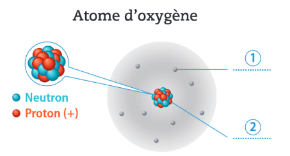
\includegraphics[width=.5\textwidth]{SchemaAtome.png}
	\caption{Schéma d'un atome.}
	% \subfloat[Schéma d'un atome]{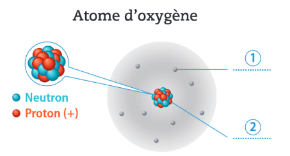
\includegraphics[width=.4\textwidth]{SchemaAtome.png}}
	% \subfloat[Isotopes]{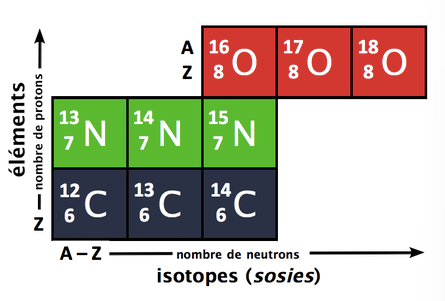
\includegraphics[width=.4\textwidth]{isotopes.png}}
	% \caption{Schéma d'un atome.}
\end{figure}

\textbf{L'atome est essentiellement constitué de vide. On dit que sa structure est lacunaire.}\medskip

\begin{minipage}{3cm}%{.3\textwidth}
\Huge{\isotope{A}{Z}{X}}
\end{minipage}
\begin{minipage}{13cm}%{.7\textwidth}
	\begin{definition}{}
		
	\begin{itemize}
		\item A est le nombre de masse, il correspond au nombre de nucléons;
		\item Z est le numéro atomique, il correspond au nombre de protons;
		\item N est le nombre de neutrons dans le noyau. 
	\end{itemize}
	
\end{definition}
\end{minipage}\medskip

Comme A correspond au nombre de nucléons, c'est à dire le nombre de protons Z et le nombre de neutrons N, il vient : 
\begin{eqnarray}
	A = N + Z.
\end{eqnarray}

\begin{definition}{Définition: élément chimique}
	% \bigskip

	L'élément chimique désigne les atomes et les ions qui possèdent le même numéro atomique Z, c'est à dire le même nombre de protons.
	% \dotfill \bigskip

	% \dotfill
\end{definition}

\begin{wrapfigure}[5]{r}{.4\textwidth}
	\vspace{-.5cm}
	\centering
	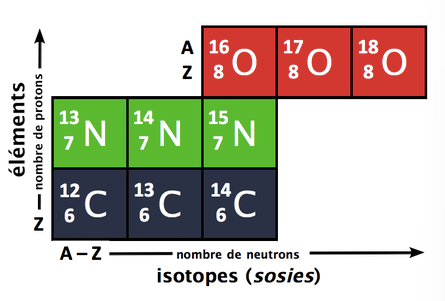
\includegraphics[width=.4\textwidth]{isotopes.png}
	\caption{isotopes [Wikipedia]}
\end{wrapfigure}

Par conséquent un élément chimique est caractérisé par le numéro atomique. C'est le numéro atomique qui va déterminer la position de l'élément dans le tableau périodique des éléments ou tableau de Mendeleïev (voir TP 3).\medskip

\begin{definition}{Définition: isotopes}
	Deux atomes qui ont le même nombre de protons mais un nombre de nucléons différents sont appelés \textbf{isotopes}. Deux atomes qui ont le même nombre de protons mais un nombre de neutrons différents sont des isotopes.
\end{definition}
\vspace{.5cm}

\begin{Exercice}{Exercices sur la représentation symbolique}
	Pour chaque Z, écrivez à quel atome X cela correspond, le numéro atomique, le nombre de protons le nombre d'électrons, et le nombre de neutrons. ainsi que sa représentation symbolique.
	\begin{multicols}{3}
		1. Z = 7; %X = N; numéro atomique = nombre de protons =7; le nombre d'électrons =7;  N=A-Z = 14-7 = 7.

		2. Z = 26; %X = Fe; numéro atomique = nombre de protons =26; le nombre d'électrons =26;  N=A-Z = 56-26 = 20.

		3. Z = 47; %X = Ag; numéro atomique = nombre de protons =47; le nombre d'électrons =47;  N=A-Z = 107-47 = 60.
	\end{multicols}
	 \vspace{3cm}
\end{Exercice}

\subsection{La masse d'un atome}

On suppose que la masse du cortège électronique est négligeable par rapport à celle du noyau de l'atome. Dans ce cas la masse notée $m$ d'un atome est pratiquement égale à celle de son noyau:

\begin{definition}{Masse d'un atome}
	\begin{equation}
		m_{\rm atome} = A\times m_{\text{nucléson}}
	\end{equation}
	\begin{itemize}
		\item Avec $m_{\rm atome}$ la masse de l'atome et $m_{\rm \text{nucléons}}$ la masse d'un nucléons en kilogramme (kg);
		\item A le nombre de nucléons dans le noyau.
	\end{itemize}
\end{definition}


\begin{Exercice}{Exercice:  Déterminer la masse d'un atome}
	\textbf{Calculer la masse d'un atome de Fer \isotope{55}{26}{Fe}}
	
	%$A=55$, donc $m_{\rm fer} = 55\times 1.675\times 10^{-27} = 9.2\times 10^{-26}$ kg.
	\vspace{2cm}
\end{Exercice}

\clearpage
\section*{Activité documentaire sur l'histoire d'un modèle, le modèle de l'atome}

\begin{mdframed}[style=doc, leftmargin=0pt, rightmargin=0pt, innertopmargin=8pt, innerbottommargin=8pt, innerrightmargin=10pt, innerleftmargin=10pt]
	\noindent\textbf{Document 1: Les recherches sur la matière}

\textbf{Vidéo:\url{https://www.youtube.com/watch?v=fhaZeqzTVjo}}
\end{mdframed}

\begin{mdframed}[style=doc, leftmargin=0pt, rightmargin=0pt, innertopmargin=8pt, innerbottommargin=8pt, innerrightmargin=10pt, innerleftmargin=10pt]
	\noindent\textbf{Document 2: Historique des recherches}
\begin{enumerate}
	\item  1804 : En étudiant le comportement des gaz, John Dalton reprend une idée de la Grèce antique longtemps abandonnée : la matière est composée de petits grains insécables appelés alors atomos;
	\item  1897 : Découverte de l'électron qui est une particule chargée négativement par John Thomson. Il propose pour l'atome un modèle de sphère de structure positive parsemée d'électrons
	\item 1911 : Découverte du noyau atomique chargé positivement et beaucoup plus petit que l'atome par Rutherford. Il propose un modèle où les électrons sont répartis dans un nuage autour du noyau mais à distance de celui-ci
	\item 1913 : Unification des théories de Max Planck et Ernest Rutherford par Niels Bohr. Il propose un modèle de répartition des électrons en couches.
	\item 1914 : Confirmation de la quantification des échanges d'énergie dans la matière par James Franck et Gustav Hertz.
\end{enumerate}

\end{mdframed}


\begin{mdframed}[style=doc, leftmargin=0pt, rightmargin=0pt, innertopmargin=8pt, innerbottommargin=8pt, innerrightmargin=10pt, innerleftmargin=10pt]

\noindent\textbf{Document 2 : Les différents modèles de l'atome}

\begin{minipage}{7cm}
	\centering
	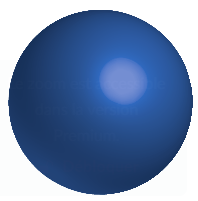
\includegraphics[width=.4\textwidth]{spheredure.png}
	\captionof{figure}{Sphère dure pleine et indivisible}
\end{minipage}\hspace{1cm}
\begin{minipage}{7cm}
	\centering
	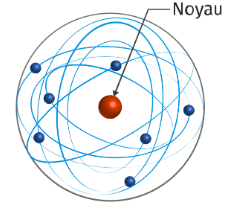
\includegraphics[width=.45\textwidth]{noyauorbite1.png}
	\captionof{figure}{Noyau positif avec des électrons qui orbitent autour. Entre les deux du vide.}
\end{minipage}\\
\begin{minipage}{7cm}
	\centering
	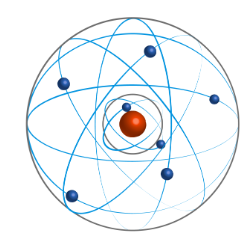
\includegraphics[width=.5\textwidth]{noyauorbite2.png}
	\captionof{figure}{Noyau positif avec des électrons qui orbitent autour. les orbites sont à des distances définies et on les appelles couches. Entre les deux du vide.}
\end{minipage}\hspace{1cm}
\begin{minipage}{7cm}
	\centering
	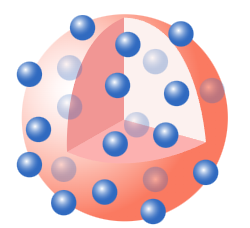
\includegraphics[width=.45\textwidth]{NoyauMatierebille.png}
	\captionof{figure}{PlumPudding, atome globalement neutre avec des électrons négatifs qui baignent dans un volume chargé positivement.}
\end{minipage}
% \begin{figure}[ht]
	% {\centering
	% 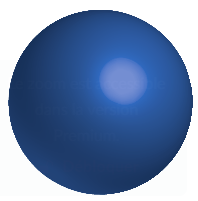
\includegraphics[width=.2\textwidth]{spheredure.png}\hspace{2cm}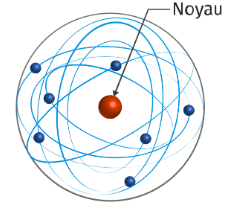
\includegraphics[width=.2\textwidth]{noyauorbite1.png}
	% \captionof{figure}{À gauche: le modèle de la sphère dure pleine et indivisible. À droite : Noyau positif avec des électrons qui orbitent autour. Entre les deux du vide.}
	% }
	
	% \subfloat[Sphère dure pleine et indivisible]{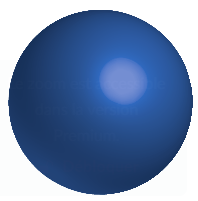
\includegraphics[width=.2\textwidth]{spheredure.png}}\hspace{3cm}
	% \subfloat[Noyau positif avec des électrons qui orbitent autour. Entre les deux du vide.]{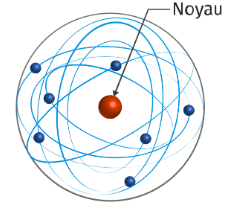
\includegraphics[width=.25\textwidth]{noyauorbite1.png}}\\
	% \subfloat[Noyau positif avec des électrons qui orbitent autour. les orbites sont à des distances définies et on les appelles couches. Entre les deux du vide.]{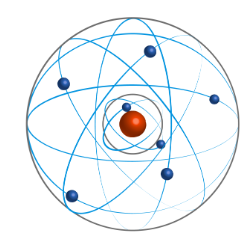
\includegraphics[width=.25\textwidth]{noyauorbite2.png}}\hspace{3cm}
	% \subfloat[PlumPudding, atome globalement neutre avec des électrons négatifs qui baignent dans un volume chargé positivement.]{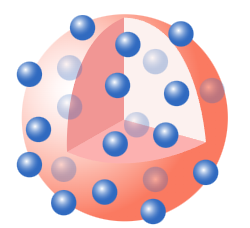
\includegraphics[width=.25\textwidth]{NoyauMatierebille.png}}
% \end{figure}

\end{mdframed}

\noindent\textbf{Questions:} 

\begin{enumerate}
	\item Associer chaque modèle à son inventeur en justifiant son choix;
	\item Faire une frise chronologique sur laquelle apparaît chaque modèle et le nom de son ou ses inventeurs
	\item Identifier la raison qui a poussé John Thomson à remettre en cause le modèle antique (Démocrite) et de John Dalton;
	\item Pourquoi le modèle de Bohr a-t-il été préféré à celui de Rutherford ? 
	\item Rappeler les étapes de la démarche scientifique. En quoi celui du modèle de l'atome est un exemple ? 
\end{enumerate}


% Quelques document vidéos intéressants. Le petit bonhomme d'IBM \url{https://www.youtube.com/watch?v=oSCX78-8-q0}.Pour résumer cette partie du cours vous pouvez regarder la vidéo suivante jusqu'à 4m37 \url{https://www.youtube.com/watch?v=gVNh_PyrWfY}




\clearpage
\section{Le cortège électronique} 


Le cortège électronique de l'atome contient l'ensemble des électrons, il définit les propriétés chimiques de l'atome.


\subsection{Une répartition en couches}

\begin{definition}{Définition: état fondamental}
% L'état fondamental d'un atome est celui pour lequel son cortège électronique (c'est à dire l'ensemble des ses électrons) est de plus bas niveau d'énergie.	
\bigskip

\dotfill \bigskip

\dotfill
\end{definition}

Les électrons d'un atome sont répartis dans des \textbf{couches électroniques}.
\begin{itemize}
	\item Chaque couche est caractérisée par un nombre entier $n>0$. 
	Par exemple $n=1,2,3,\dots$ 
	

	\item Chaque sous-couche est caractérisée par un entier $l$ tel que : $0\leq l < n$
\end{itemize}


\begin{wrapfigure}[14]{r}{.4\textwidth}
	\centering
	% \vspace{-4cm}
	% 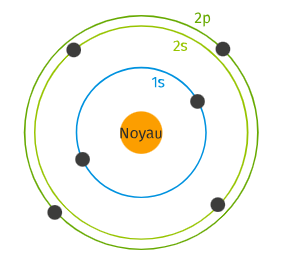
\includegraphics[width=.3\textwidth]{ModeleAtome.png}
	\begin{tikzpicture}[scale=0.6]
		\draw[fill=gray!20] (0,0) circle (0.5);
		\draw  (0,0) node{$+$};
		\draw[dashed, color=definitionl] (0,0) circle (1);
		\draw[color = definitionl] (1.1,.7) node{$1s$};
	
		\draw[dashed, color=red] (0,0) circle (1.7);
		\draw[color = red] (.8,1.3) node{$2s$};
	
		\draw[dashed, color=red!40] (0,0) circle (2.1);
		\draw[color = red!40] (.9,2.2) node{$2p$};
	
		\draw[dashed, color=blue] (0,0) circle (3.8);
		\draw[color = blue] (1,3.3) node{$3s$};
	
		\draw[dashed, color=blue!40] (0,0) circle (4.2);
		\draw[color = blue!40] (1.3,4.4) node{$3p$};
		
		% \draw (-3,-4.1) node{\textcolor{blue}{\textbf{Légende:}}};
		% \draw[fill=gray!20] (-3,-5) circle (0.5);
		% \draw  (-3,-5) node{$+$};
		% \draw  (-1.5,-5) node{Noyau};
		% \draw[dashed] (-3,-6)--(-2.5,-6) node[right]{sous-couches électroniques};
	
	\end{tikzpicture}
	\caption{Modèle de l'atome de carbone}
\end{wrapfigure}
Chaque sous-couche porte un nom, la couche "s" correspond à $l=0$, la couche "p" correspond à $l=1$ et la couche "d" à $l=2$.  Pour les atomes de numéro atomique $Z\leq 18$, les électrons sont répartis dans des couches nommées \textbf{ns, np}.\medskip

\noindent Exemple :

\begin{itemize}
	\item Si $n = 1, l=0$. Cela correspond à la couche électronique que l'on notera "1s". 
	\item Si $n = 2, l=[0,1]$. Ces deux couches électroniques s'écrivent "2s2p".
	\item Si $n=3, l= [0,1,2]$. Ces couches électroniques s'écrivent "3s3p3d". 
\end{itemize}

\textbf{Remarque:} Il en existe d'autres afin de décrire l'ensemble des atomes du tableau périodique. Mais on se restreint à ces trois premières couches électroniques dans le cadre du programme de seconde.

\subsection{Remplissage des couches électroniques}
Les électrons se répartissent sur les différentes couches et sous-couches suivant des règles précises chaque sous-couche peut contenir un nombre d'électrons \textbf{maximum} qui lui est propre.

\begin{definition}{Configuration électronique}
	\begin{wrapfigure}{r}{.4\textwidth}
		\centering
		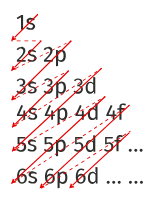
\includegraphics[width=.2\textwidth]{Klechkowski.png}
		\caption{Règle de Klechkowski}
	\end{wrapfigure}
	\bigskip

	\dotfill \bigskip
	
	\dotfill \bigskip

	\dotfill \bigskip

	\dotfill
	% On appelle la \textbf{configuration électronique} de l'atome la répartition des électrons dans des couches et sous-couches électroniques. Les sous-couches se remplissent selon l'ordre suivant (règle de Klechkowski): 
	% \[1s\rightarrow 2s \rightarrow 2p \rightarrow 2p \rightarrow 3s \rightarrow 3p\] 

	\begin{itemize}
		\item Une sous-couche de type \textbf{s} ($l=0$) peut contenir \textbf{deux électrons};
		\item Une sous-couche de type \textbf{p} (l=1) peut contenir jusqu'à \textbf{six électrons}.
	\end{itemize}
\end{definition}

Écrire la configuration élecrtonique d'un atome à l'état fondamental coniste à écrire l'ensemble des noms de tous ses électrons. Dans cette écriture les nombres d'électrons s et p sont indiqués en exposant.\medskip

\clearpage
\noindent \textbf{Exemple}: la configuration électronique de l'atome de phosphore \isotope{31}{15}{P} (Z = 15) à l'état fondamental est :\bigskip 

% \dotfill \bigskip

\[ \rm (1s)^2(2s)^2(2p)^6(3s)^2(3p)^3\]
\begin{table}[ht]
	\centering
	\begin{tabular}{|c|c|c|c|c|c|}
		\hline 
		\textbf{Sous-couche électronique} & 1s & 2s & 2p & 3s & 3p \\ \hline
		\textbf{Nombre d'électrons ns ou np} & 2 & 2 & 6 & 2 & 6 \\ \hline 
	\end{tabular}
\end{table}


\begin{definition}{Définition : Les électrons de c\oe ur et de valence}
	\bigskip
	
	\dotfill \bigskip

	\dotfill \bigskip

	\dotfill

	% La dernière couche contentant des électrons est appelée \textbf{couche externe} ou \textbf{couche de valence}. Elle contient les \textbf{électrons de valence}.\bigskip
	
	% Les autres couches sont appelées \textbf{couches internes}. Elles contiennent les \textbf{électrons de c\oe ur} des atomes.
\end{definition}

\noindent \textbf{Exemple:} Le phosphore \isotope{31}{15}{P} a pour configuration électronique : \[\rm \underbrace{(1s)^2(2s)^2(2p)^6}_{\text{couche interne}}\underbrace{(3s)^2(3p)^3}_{\text{couche externe}}\] 
Il possède $2+2+6=10$ électrons de c\oe ur et $2+3=5$ électrons de valence.

\subsection{Lien entre la configuration électronique et  le tableau périodique}

La classification périodique s'est construite par tâtonnement au XIX$^{\rm e}$ siècle jusqu'à la version actuelle dont la base est celle de \textbf{Dmitri Mendeleïev} en 1869.\medskip


Le tableau périodique regroupe les éléments chimiques qui y sont rangés en fonction des configurations électroniques de leurs atomes à \textbf{l'état fondamental}. La configuration électronique d'un atome à l'état fondamental permet de déterminer sa position dans le tableau périodique.\bigskip

\begin{definition}{Critère de classification}
Les éléments chimiques sont classés en lignes par numéro atomique croissant. Le remplissage progressif d'une ligne correspond au remplissage progressif d'une couche électronique. Un changement de ligne s'effectue lorsqu'une nouvelle couche commence à se remplir.\bigskip

\begin{itemize}
	\item \dotfill \bigskip
	
\dotfill \bigskip
	
	\item \dotfill \bigskip
	
\dotfill \bigskip

	% \item La valeur de $n$ des électrons de valence détermine la ligne dans laquelle se situe l'atome. Cette valeur correspond au niveau de la ligne. 
	% \item Le nombre d'électrons de valence détermine la colonne dans laquelle se situe l'atome. Ce nombre correspond au chiffre des unités du numéro de la colonne.
\end{itemize}
\end{definition}\bigskip

\begin{Exercice}{Exercice : Déterminer la position de l'atome de phosphore}

	% Dans le cas de l'atome de phosphore, les électrons de valence se trouvent sur les couches 3s 3p. Donc n = 3, il appartient à la troisième ligne. Comme Z= 15, il se trouve sur la $15^{\rm e}$ colonne du tableau périodique. Les électrons $3p$ indiquent que le phosphore appartient à la 3eme colonne du bloc p.
	\medskip 

	\dotfill \medskip

	\dotfill \medskip

	\dotfill
\end{Exercice}


\begin{definition}{Défintion : Famille chimique}

Les éléments chimiques d'une même colonne dans le tableau périodique constituent une \textbf{famille chimique}.  Ils ont :

\begin{itemize}
	\item \dotfill \bigskip
	
	\item \dotfill 
	% \item le le même nombre d'électrons sur leur couche externe \textbf{électrons de valence}
	% \item  les mêmes propriétés chimiques. 
\end{itemize}

\end{definition}

\begin{Exercice}{Exercices}
	Savoir faire : écrire les configurations électronique et retrouver des éléments dans le tableau périodique.

	\begin{itemize}
		\item Exercices 12,13 p. 98
		\item Exercices 15p.99
	\end{itemize}
\end{Exercice}
\section{Vers des entités plus stables}

\subsection{Les gaz nobles}
Dans la nature, les atomes ont tendance à s'associer pour former des molécules. Seuls les atomes de la colonne n$^\circ 18$ appelés gaz nobles (He, Ne, Ar, Kr, etc) présentent une grande inertie chimique: ce sont des gaz monoatomiques dans les conditions ordinaire de température et de pression ($T=20^\circ \rm C$ $P = 1~\rm  bar$).  Cette particularité est liée à la configuration électronique de la couche externe des atomes constituant cette famille chimique. 


\begin{Exercice}{Écrire les configurations électroniques de l'hélium \isotope{4}{2}{He}, du néon \isotope{20}{10}{Ne} et de l'argon \isotope{40}{18}{Ar}}.\smallskip

\begin{itemize}
	\item He (Z=2): \dotfill\bigskip %$\rm (1s)^2$;
	\item Ne (Z=10): \dotfill\bigskip%$\rm (1s)^2(2s)^2(2p)^6$;
	\item Ar (Z=18): \dotfill\bigskip%$\rm (1s)^2(2s)^2(2p)^6(3s)^2(3p)^6$
\end{itemize} 
\end{Exercice}
\begin{definition}{Règles de stabilité}
	La grande stabilité des gaz nobles est liée au nombre d'éléctrons qu'ils possèdent sur leur couche externe. 
\begin{itemize}
	\item Pour l'atome d'hélium : \dotfill\medskip%soit deux électrons ou duet pour l'atome d'Hélium;
	\item Pour les autres atomes : \dotfill\medskip% soit huit électrons ou un octet pour les autres atomes.
\end{itemize}
\end{definition}

\subsection{Les ions monoatomiques}

Les atomes des colonnes 1,2,4, 15,16, 17 du tableau périodique tendent à perdre ou à gagner des électrons pour former un ion monoatomique ayant autant d'électrons que l'atome de gaz noble le plus proche en numéro atomique.

% \begin{table}[ht]
% 	\centering
% 	\begin{tabular}{|c|c|c|c|c|}
% 		\hline 
% 		\textbf{Formule de l'ion} & $\rm H^+$ & $\rm Na^+$ & $\rm K^+$ & $\rm Mg^{2+}$ \\ \hline
% 		\textbf{Nom de l'ion} & hydrogène & sodium & potassium & magnésium \\ \hline 
% 	\end{tabular}
% \end{table}

\begin{table}[ht]
	\centering
	\begin{tabular}{|c|c|c|c|c|c|}
		\hline 
		\textbf{Formule de l'ion} & $\rm H^+$ & $\rm Na^+$ & $\rm K^+$ & $\rm Mg^{2+}$ \\ \hline
		\textbf{Nom de l'ion} &  &  &  & \\ \hline 
	\end{tabular}
\end{table}
\subsection{Liaison covalente et schéma de Lewis}

Dans les molécules, les atomes mettent en commun des électrons afin de gagner en stabilité.

\begin{definition}{Définition : La liaison covalente}
% \textbf{La liaison covalente} est une mise en commun de deux électrons de valence entre deux atomes. Elle peut être simple, double ou triple. 
\bigskip

\dotfill \bigskip

\dotfill
\end{definition}
On représente une liaison covalente par un tiret entre les deux atomes concernés:
\begin{center}
\chemfig[atom sep =2em]{A-B}\hspace{3cm} \chemfig{A=B}\hspace{3cm} \chemfig{A~B}
\end{center}

Les électrons de valence d'un atome qui \textbf{ne participent pas} aux liaisons covalentes sont répartis en doublets d'électrons appelés \textbf{doublets non liants}. Chaque doublet non liant est représenté par un tiret placé sur l'atome considéré.

\begin{center}
	\chemfig[atom sep =2em]{A-\charge{90=\|}{B}}
\end{center}


Chaque atome respectera donc soit la règle du duet, soit la règle de l'octet. Les formules de Lewis des molécules permettent de vérifier le respect de ces règles en comptabilisant les électrons des liaisons covalentes et des doublets non liants pour chaque atome de la molécule.

\begin{Exercice}{Exercice : Déterminer la formule de Lewis de l'eau $H_2O$}
\begin{enumerate}
	\item Donner la configuration électronique de l'oxygène $O$ et de l'hydrogène.
	\item Combien d'électrons de valence sont mis en jeu ? 
	\item Représenter la formule de Lewis de l'eau.
\end{enumerate}

\end{Exercice}



\begin{figure}[ht]%{r}{.5\textwidth}
	\centering
	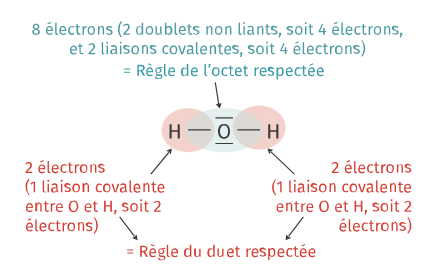
\includegraphics[width=.5\textwidth]{FormuleDeLewis.png}
	\caption{Formule de lewis de l'eau.}
\end{figure}

\begin{definition}{Définition : Énergie de laison}

L'énergie de liaison $\mathcal{E}_{AB}$ entre deux atomes A et B liés dans une molécule est l'énergie que doit recevoir cette molécule pour rompre la liaison AB, chaque entité A et B formée gardant avec elle la motié des électrons des douvlets liants rompus. 

\end{definition}
\begin{Exercice}{Exercices}
	\begin{itemize}
		\item Configuration électronique et règle de l'octet : Exercie 5,7, 8 p115
		\item Stabilité : Exercice 10p115
		\item Représentations de Lewis : 15p116
		\item Liaisons covalentes Structure : 21 p 118
	\end{itemize}


\end{Exercice}
\end{document}

%%
%% FIN DU DOCUMENT
%%
